\section{Вычисление факториала}
\subsection{Условие задания}
Разработать приложение для вычисления факториала по приведённому примеру.

Приложение должно содержать следующие компоненты:

\begin{enumerate}
  \item Заголовок формы должен отражать суть задания.
  \item Все элементы формы должны быть внятно подписаны (кнопки подписаны, у текстового поля должно быть написано, для чего оно нужно и т.д.)
  \item В коде должны быть комментарии и отступы (код должен быть легко читаем).
  \item В коде программы все элементы формы должны быть переименованы (btnName -  для кнопок, lblName - для ссылок, txtName - для текстового поля и т. д.) Наименования должны быть понятными.
  \item Приложение должно корректно работать (выводить ответ или ошибку с соответствующим сообщением) для следующих данных: ввод буквы, ввод отрицательного числа, ввод нуля, ввод положительного числа (< 10), ввод большого положительного числа. После вывода ошибок при вводе корректных данных поля ошибок должны очищаться.
\end{enumerate}

\subsection{Факториал натурального числа}
Факториалом натурального числа $n$ называют число $n!$, такое, что:

\begin{equation}
  n! = 1 \times 2 \times \dots \times (n - 1) \times n
\end{equation}

\subsection{Нахождение факториала рекурсивным способом}
Пусть на вход подано число $n\in\mathbb{N}$. Тогда алгоритм \cite{factorial-calculation} будет выглядеть таким образом:
\begin{itemize}
  \item Если $0 \leqslant n \leqslant 1$, то возвращаем $0! = 1! = 1$;
  \item Если $n > 1$, то возвращаем $n! = (n-1)!\times n$.
\end{itemize}
Таким образом, мы можем рекурсивно вычислить факториал любого достаточно малого числа $n$. Для больших чисел алгоритм будет медленным в силу экстремально быстрого роста функции факториала.

\subsection{Вид формы в конструкторе}
Форма имеет вид:
\begin{figure}
  \centering
  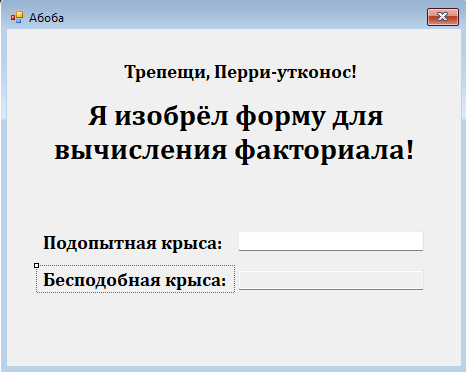
\includegraphics[width=0.5\linewidth]{images/factorial/form.png}
  \caption{Форма окна для вычисления факториала}
  \label{fig:factorial-form}
\end{figure}

\subsection{Таблица с описанием элементов формы}
Все элементы формы были переименованы для большей читаемости. В таблице \ref{tab:factorial-form} представлены все изменения.

\begin{table}
  \centering
  \begin{tabular}{|m{0.3\textwidth}|m{0.3\textwidth}|m{0.3\textwidth}|}
    \hline
    \textbf{Описание элементов формы} & \textbf{Список изменённых атрибутов} & \textbf{Новое значение атрибута} \\
    \hline
    \hline
    Окно формы & Text & Абоба \\
    Верхний подзаголовок & Name & lblSubtitle \\
    Верхний заголовок & Name & lblTitleStart \\
    Нижний заголовок & Name & lblTitleEnd \\
    Метка поля ввода & Name & lblInput \\
    Метка поля вывода & Name & lblOutput \\
    Поле ввода & Name & textInput \\
    Поле вывода & Name & textOutput \\
    \hline
  \end{tabular}
  \caption{Значение атрибутов элементов в приложении для вычисления факториала}
  \label{tab:factorial-form}
\end{table}

\subsection{Примеры правильной и неправильной работы приложения}
При запуске приложения на экране появляется окно \ref{fig:factorial-start}.
\begin{figure}
  \centering
  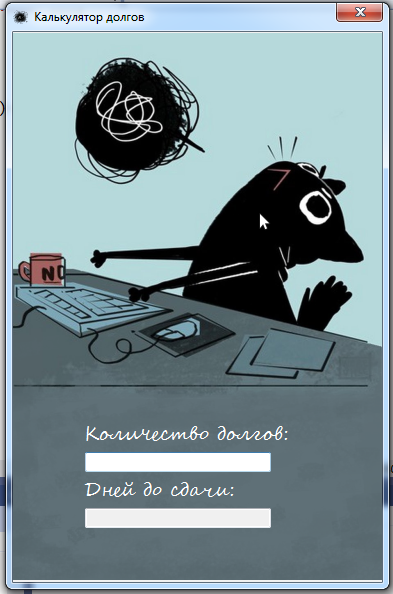
\includegraphics[width=0.5\linewidth]{images/factorial/start.png}
  \caption{Запуск программы}
  \label{fig:factorial-start}
\end{figure}

При вводе реактивно подсчитывается и подставляется значение в поле вывода. Также реактивно происходит обработка ошибок.

\begin{figure}
  \centering
  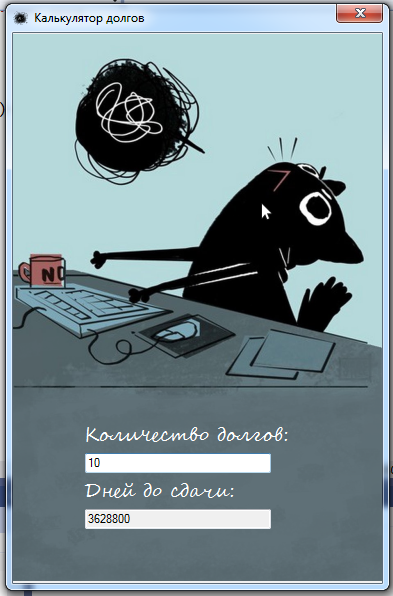
\includegraphics[width=0.5\linewidth]{images/factorial/okay.png}
  \caption{Запуск программы с корректными данными}
  \label{fig:factorial-okay}
\end{figure}

\begin{figure}
  \centering
  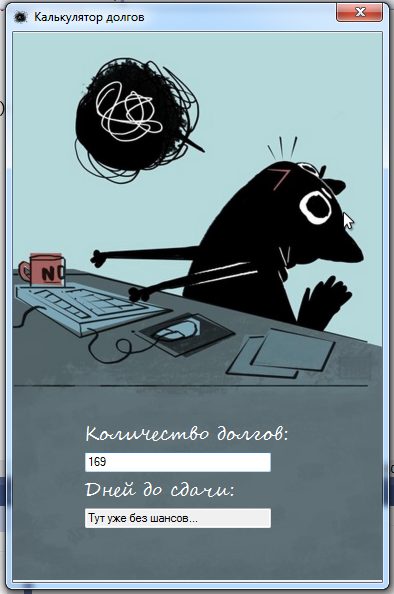
\includegraphics[width=0.5\linewidth]{images/factorial/error.png}
  \caption{Запуск программы с некорректными числовыми данными}
  \label{fig:factorial-error}
\end{figure}

\begin{figure}
  \centering
  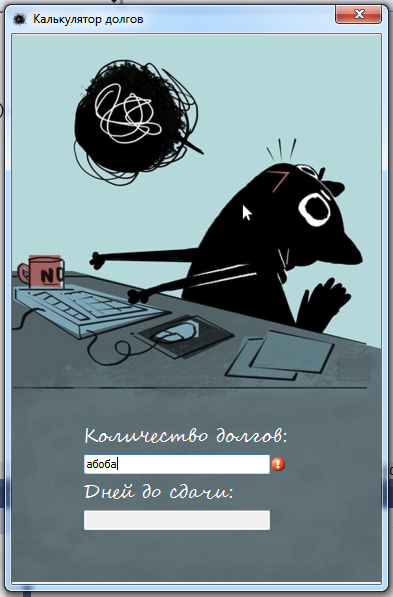
\includegraphics[width=0.5\linewidth]{images/factorial/error2.png}
  \caption{Запуск программы с нечисловыми данными}
  \label{fig:factorial-error2}
\end{figure}

\subsection{Примеры исходного кода}
\begin{minted}{cpp}
/* Процедура для очистки экрана */
private: void ClearAll() {
  this->textOutput->Text = "";
  errorProvider->SetError(textInput, String::Empty);
}

/* Обработчик события изменения текстового поля */
private: System::Void textInput_onChange(System::Object^ sender, System::EventArgs^ e) {
  ClearAll();
  long long InputNumber;
  bool result = Int64::TryParse(this->textInput->Text, InputNumber);

  // в result записали булеву переменную, отвечающую за корректный ввод
  if (!result)
    errorProvider->SetError(textInput, "Введено не целое число");
  else {
    // по условию задачи число не должно быть больше 20
    if (InputNumber > 20)
      this->textOutput->Text = "Слишком большое число";
    else {
      // внешняя рекурсивная функция факториала вернёт -1 только в одном случае -- если исходное число отрицательное
      long long OutputNumber = factorial(InputNumber);
      if (OutputNumber == -1)
        errorProvider->SetError(textInput, "Введено отрицательное число");
      else this->textOutput->Text = System::Convert::ToString(OutputNumber);
    }
  }
}
\end{minted}

Больше кода проекта доступно в приложении \ref{application-A}. Также в приложенном архиве можно найти полный код проекта.